% Gemini theme
% https://github.com/anishathalye/gemini

% !TEX program = lualatex
\documentclass[final]{beamer}

% ====================
% Packages
% ====================

\usepackage[T1]{fontenc}
\usepackage{lmodern}
\usepackage[size=custom,width=36,height=48,scale=0.4]{beamerposter}
\usetheme{gemini}
\usecolortheme{mit}
\usepackage{graphicx}
\usepackage{booktabs}
\usepackage{tikz}
\usepackage{pgfplots}

% ====================
% Lengths
% ====================

% If you have N columns, choose \sepwidth and \colwidth such that
% (N+1)*\sepwidth + N*\colwidth = \paperwidth
\newlength{\sepwidth}
\newlength{\colwidth}
\setlength{\sepwidth}{0.02\paperwidth}
\setlength{\colwidth}{0.42\paperwidth}

\newcommand{\separatorcolumn}{\begin{column}{\sepwidth}\end{column}}

% ====================
% Title
% ====================

\title{Assessment of Tethered Balloon-Borne Observations \\ of Arctic Low Cloud Properties}

\author{GUNHO (LOREN) OH \inst{1} \and SANGJONG PARK \inst{1}}

\institute[shortinst]{\inst{1} Korean Polar Research Institute (KOPRI)}

% ====================
% Footer (optional)
% ====================

\footercontent{
Korea Polar Research Institute (KOPRI), Incheon, Korea \hfill \null
}
% (can be left out to remove footer)

% ====================
% Logo (optional)
% ====================

% use this to include logos on the left and/or right side of the header:
% \logoright{\includegraphics[height=7cm]{logo1.pdf}}
% \logoleft{\includegraphics[height=7cm]{logo2.pdf}}

% ====================
% Body
% ====================

\begin{document}

\begin{frame}[t]
  \begin{columns}[t]

    \separatorcolumn
    \begin{column}{\colwidth}

      \begin{block}{Abstract}
        Low-altitude clouds exert a major influence on the radiative energy budget in the Arctic region. Studies have shown that Arctic clouds contribute to warming of the surface through long-wave cloud radiative effect, except during the peak of summer when the cooling effect due to their high albedo dominates. Although low-altitude clouds remain one of the largest uncertainties in modelling the Arctic climate, our understanding of the thermodynamic processes governing these clouds remains incomplete. In-situ observations of cloud properties are scarce, and uncertainties involved in remote sensing observations make it difficult to precisely determine the cloud properties and the thermodynamic state of the atmosphere. To this end, we make a comparison between an in-situ observation of the low-altitude clouds using a cloud particle detector, and measurements taken from a ground-based remote sensing site (retrieved from CloudNet). We examine the measurements taken from the Backscatter Cloud-probe with Polarization Detection (BCPD) mounted on a tethered balloon to obtain the cloud properties such as liquid water content (LWC), size-resolved number concentration (NC) and size distribution. The results from the  observation are used to examine the assumptions made in estimating the properties of the mixed-phase clouds from the remote sensor measurements.
      \end{block}

      \begin{block}{Methods}
        A Backscatter Cloud Probe (BCPD) was mounted on a tethered balloon instrument on October 1st, 2019, near Ny-\r{A}lesund, Svalbard, in order to measure thermodynamic properties of low-altitude mixed-phase clouds.

        \begin{figure}
          \centering
          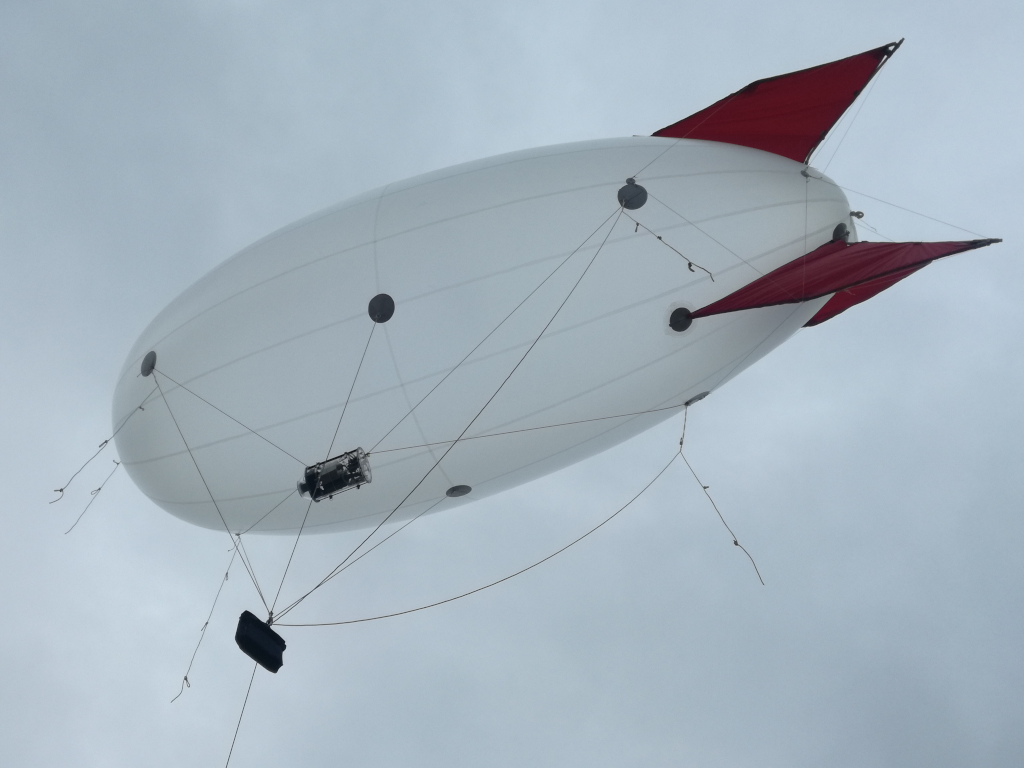
\includegraphics[width=0.8\colwidth]{figure/balloon.png}
          \caption{A photo of the Backscatter Cloud Probe (BCPD) mounted on a tethered balloon, deployed on October 1st, 2019 near Ny-\r{A}lesund, Svalbard.}
        \end{figure}
      \end{block}

      \begin{figure}
        \centering
        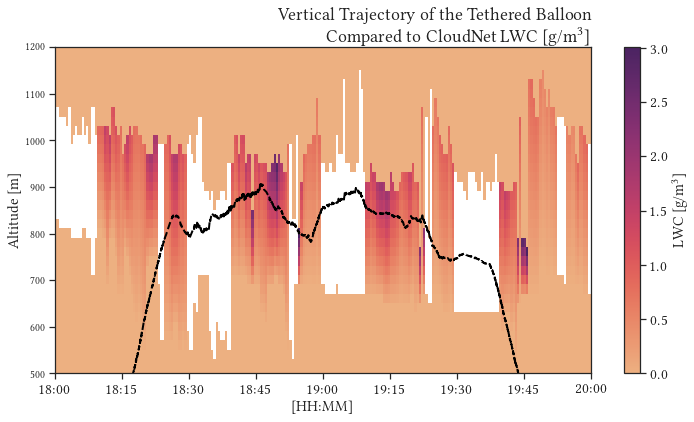
\includegraphics[width=\colwidth]{figure/ts_alt.png}
        \caption{A figure caption.}
      \end{figure}

    \end{column}

    \separatorcolumn
    \begin{column}{\colwidth}

      \begin{alertblock}{Results}
        The following figures show some of the primary microphysical properties reported by BCPD.

        \begin{figure}
          \centering
          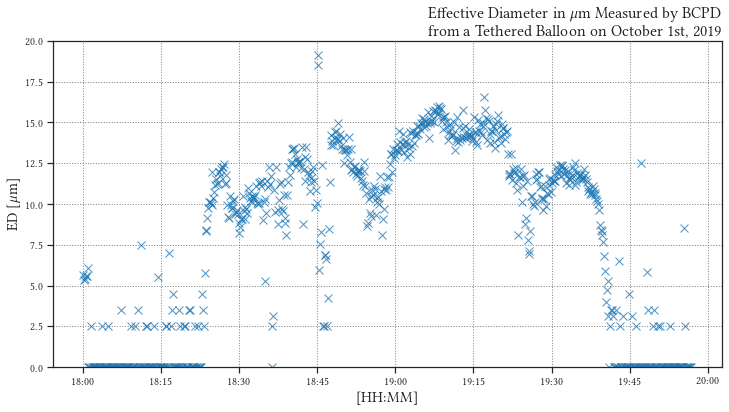
\includegraphics[width=\colwidth]{figure/ts_ed.png}
          \caption{A figure caption.}
        \end{figure}

        \begin{figure}
          \centering
          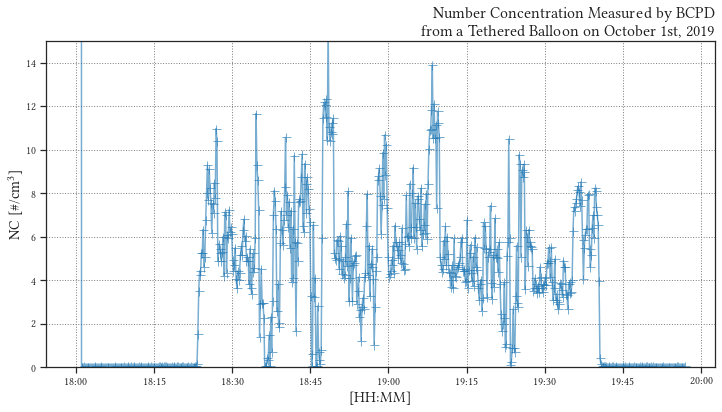
\includegraphics[width=\colwidth]{figure/ts_nc.png}
          \caption{A figure caption.}
        \end{figure}

        \begin{figure}
          \centering
          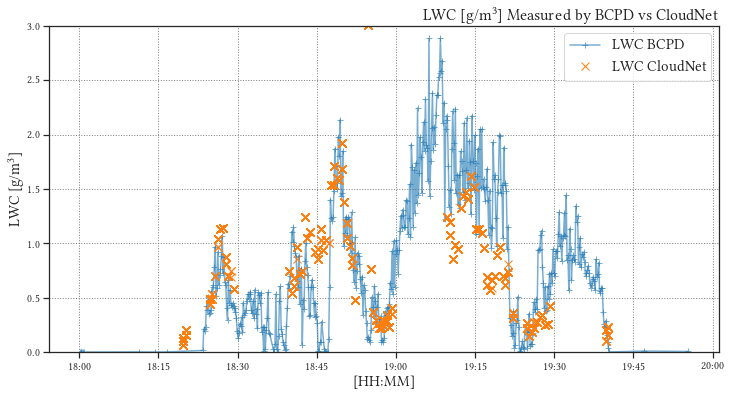
\includegraphics[width=\colwidth]{figure/ts_lwc.png}
          \caption{A figure caption.}
        \end{figure}

      \end{alertblock}

      \begin{block}{Conclusion}
        The thermodynamic properties of low-altitude mixed-phase clouds measured on Octobe 1st, 2019, corresponds well to the remote sensing observations reported by CloudNet. The in-situ observation has an added benefit of 
      \end{block}

    \end{column}

    \separatorcolumn
  \end{columns}

\end{frame}
\end{document}
